\documentclass[10pt]{article}

\usepackage[margin=0.75in]{geometry}
\usepackage{amsmath,amsthm,amssymb}
\usepackage{xcolor}
\usepackage{cancel}
\usepackage{graphicx}
\usepackage{changepage}
\usepackage{circuitikz}
\usepackage{pgfplots}
\usepackage{physics}
\usepackage{hyperref}
\usepackage{siunitx}
\usepackage{fontspec}
\usepackage{relsize}
\usepackage{subfig}
\usepackage{todonotes}
\usepackage{multicol, multirow, booktabs}
\usepackage[breakable]{tcolorbox}
\usepackage[inline]{enumitem}

\theoremstyle{definition}
\newtheorem{problem}{Problem}
\newtheorem{soln}{Solution}

\pgfplotsset{compat=newest}
\usetikzlibrary{lindenmayersystems}
\usetikzlibrary{arrows}
\usetikzlibrary{calc}
\usetikzlibrary{positioning, fit}
\usetikzlibrary{3d, perspective}

\definecolor{incolor}{HTML}{303F9F}
\definecolor{outcolor}{HTML}{D84315}
\definecolor{cellborder}{HTML}{CFCFCF}
\definecolor{cellbackground}{HTML}{F7F7F7}
\newcommand{\ui}{\hat{i}}
\newcommand{\uj}{\hat{j}}
\newcommand{\uk}{\hat{k}}
\newcommand{\ux}{\hat{\mathbf{x}}}
\newcommand{\uy}{\hat{\mathbf{y}}}
\newcommand{\uz}{\hat{\mathbf{z}}}
\newcommand{\uv}[1]{\hat{\mathbf{{#1}}}}
\newcommand{\pr}[1]{{#1^\prime}}
\pgfdeclarelayer{background}  
\pgfsetlayers{background,main}
\AtBeginDocument{\RenewCommandCopy\qty\SI}

\makeatletter
\newcommand{\boxspacing}{\kern\kvtcb@left@rule\kern\kvtcb@boxsep}
\makeatother
\newcommand{\prompt}[4]{
    \ttfamily\llap{{\color{#2}[#3]:\hspace{3pt}#4}}\vspace{-\baselineskip}
}

\newcommand{\thevenin}[2]{
  \begin{center}
    \begin{circuitikz} \draw
      (0,0) -- (2,0) to[battery1, l_=$V_{Th}\eq#1$] (2,2) 
      to[resistor, l_=$R_{Th}\eq#2$] (0,2)
      ;
      \draw [o-] (-.07,2.079);
      \draw [o-] (-.07,0.079);
    \end{circuitikz}
  \end{center}
}

\newcommand{\norton}[2]{
  \begin{center}
    \begin{circuitikz} \draw
      (0,0) -- (3,0) to[american current source, l_=$I_{N}\eq#1$] (3,2) -- (0,2) (2,0)
      to[resistor, l=$R_{N}\eq#2$] (2,2)
      ;
      \draw [o-] (-.07,2.079);
      \draw [o-] (-.07,0.079);
    \end{circuitikz}
  \end{center}
}

\DeclareMathOperator{\Div}{div}
\DeclareMathOperator{\Curl}{curl}

\newcommand{\highlight}[1]{\colorbox{yellow}{$\displaystyle #1$}}

\newcommand{\ti}[1]{\widetilde{#1}}

\newfontface{\Kaufmann}{Kaufmann}
\DeclareTextFontCommand{\kf}{\Kaufmann}
\newcommand{\scriptr}{\fontsize{12pt}{12pt}\kf{r}}

\newfontface{\KaufmannB}{Kaufmann Bd BT}
\DeclareTextFontCommand{\kfb}{\KaufmannB}
\newcommand{\bscriptr}{\fontsize{12pt}{12pt}\kfb{r}}
\newcommand{\justif}[2]{&{#1}&\text{#2}}
\newcommand{\bv}[1]{\mathbf{#1}}

\title{Physics 3200Y: Assignment III}
\author{Jeremy Favro (0805980) \\ Trent University, Peterborough, ON, Canada}
\date{\today}

\begin{document}
\maketitle

% PROBLEM 1
\begin{problem}
This question asks you to re-work the proof in Sec. 3.1.4 of your textbook. Find the average potential over a
spherical surface of radius $R$ due to a point charge $q$ located inside the surface (i.e. with $z < R$). Show that
$$
  V_{avg}=V_{centre}+\frac{Q_{enc}}{4\pi \epsilon_0}
$$
Here, $V_{avg}$ is the potential at the centre due to all external charges and $Q_{enc}$ is the total enclosed charge.
\end{problem}
\begin{soln}
  For a restatement of the setup of the proof by Griffiths we note that the potential at a point
  is the average value of the potential on a spherical surface $\mathcal{S}$ of radius $R$ centered about the point,
  $$
    V(\bv{r})=\frac{1}{4\pi R}\oint_{\mathcal{S}} V\,da.
  $$
  Because I'm a bit busy at the moment let's simplify the diagram down to a 2D picture immediately using our
  knowledge of the symmetry in this problem. As Griffiths does let's construct our coordinate system and bounding sphere so that
  the sphere is positioned at the origin and the charge $q$ is at some $\pr{\bv{r}}=\pr{z}\uz$.
  \begin{center}
    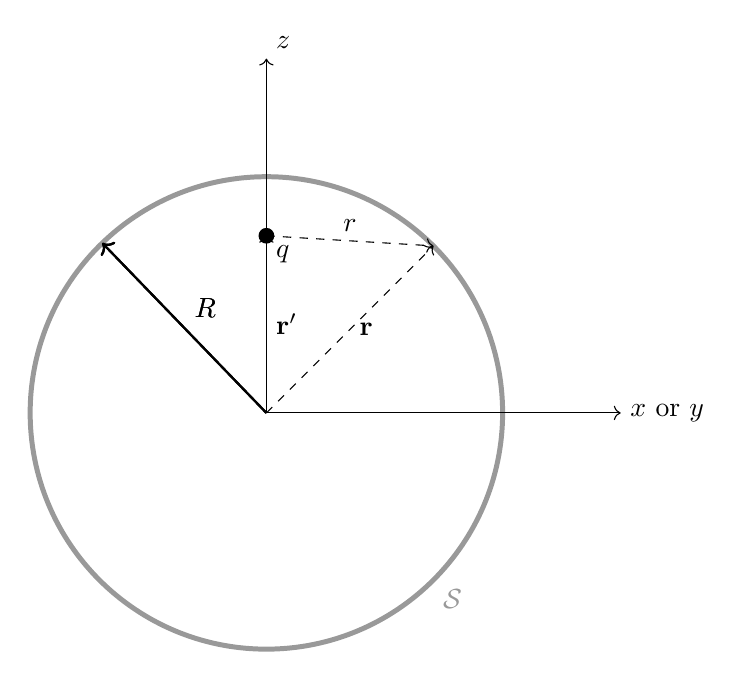
\begin{tikzpicture}
      \def\R{3}
      \def\L{4.0}
      \coordinate (Q) at (0,{3*\R/4});

      % SPHERE
      \draw[black!40, line width=1.8] (0,0) circle(\R);
      \node[black!40, below right] at ({\R/sqrt(2)}, {-\R/sqrt(2)}) {$\mathcal{S}$};

      % AXES
      \draw[->] (0,0) -- (1.5*\R,0) node[right] {$x$ or $y$};
      \draw[->] (0,0) -- (0,1.5*\R) node[above right] {$z$};
      \draw[thick, ->] (0,0) -- (134:\R) node[midway, above right] {$R$};
      \draw[thick, ->] (0,0) -- (134:\R) node[midway, above right] {$R$};

      % CHARGE
      \fill (Q) circle (0.1) node[below right] {$q$};
      \draw[->, dashed] (0,0) -- (Q) node[midway, right] {$\bv{\pr{r}}$};
      \draw[->, dashed] (0,0) -- ({\R/sqrt(2)}, {\R/sqrt(2)}) node[midway, right] {$\bv{r}$};
      \draw[->, dashed] (Q) -- ({\R/sqrt(2)}, {\R/sqrt(2)}) node[midway, above] {$\bscriptr$};

    \end{tikzpicture}
  \end{center}
  We can recognize that $\abs{\pr{\bv{r}}}=z^2$ and $\abs{\bv{r}}=R^2$. Then, labeling the angle
  between $\bv{r}$ and $\pr{\bv{r}}$ as $\theta$, we can determine $\abs{\scriptr}$ using cosine law,
  $$\abs{\scriptr}=\scriptr^2=z^2+R^2-2zR\cos\theta.$$
  Now recalling the expression for potential due to a charge $q$ is
  $$V=\frac{1}{4\pi\epsilon_0}\frac{q}{\scriptr}$$
  we can write the average potential over the sphere as
  $$V_{avg}=\frac{1}{4\pi R^2}\frac{q}{4\pi\epsilon_0}\int_{0}^{2\pi}\int_{0}^{\pi}\frac{1}{\scriptr}R^2\sin\theta\,d\theta d\phi.$$
  The $\phi$ integral just drops down to multiplication by $2\pi$ and the $\theta$ integral is a $u$ substitution
  for $u=z^2+R^2-2zR\cos\theta\implies du=2zR\sin\theta$ which gives
  $$V_{avg}=\frac{2q}{4^2zR\pi\epsilon_0}\left[z^2+R^2-2zR\cos\theta\right]_{\theta=0}^{\pi}
    =\frac{2q}{4^2zR\pi\epsilon_0}\left(\left[z^2+R^2+2zR\right]^{1/2}-\left[z^2+R^2-2zR\right]^{1/2}\right).$$
  We can rewrite the terms inside the square roots as binomials and note that $\abs{z-R}=\abs{R-z}=R-z$
  $$V_{avg}=\frac{2q}{4^2zR\pi\epsilon_0}\left(\abs{z+R}-\abs{z-R}\right)
    =\frac{2q}{4^2zR\pi\epsilon_0}\left(z+R-R+z\right)
    =\frac{q}{4\pi\epsilon_0R}$$
  We can generalize this to multiple charges inside the sphere with a total charge $Q_enc$ as electric potential obeys linear superposition,
  $$V_{avg}=\frac{Q_{enc}}{4\pi\epsilon_0R}.$$
  Finally if there are charges outside the sphere we can tack on a term, $V_{centre}$, which accounts for the contribution
  to the potential on the surface of the sphere as noted by Griffiths in the original proof:
  $$V_{avg}=V_{centre}+\frac{Q_{enc}}{4\pi\epsilon_0R}.$$
\end{soln}

% PROBLEM 2
\begin{problem}
Find the general solution to Laplace's equation in spherical coordinates for the case where $V$ depends only on
$r$. Repeat the calculation for cylindrical coordinates for the case where $V$ depends only on $s$.
\end{problem}
\begin{soln}
  From the front cover of Griffiths we have that
  $$\nabla_r^2=\frac{1}{r^2}\frac{\partial}{\partial r}\left(r^2\frac{\partial}{\partial r}\right)$$
  which gives the specific case of Laplace's equation here to be
  $$\nabla^2 V(r)=\frac{1}{r^2}\frac{\partial}{\partial r}\left(r^2\frac{\partial V}{\partial r}\right)=0.$$
  Provided $r\neq 0$ we can eliminate the $1/r^2$,
  $$\frac{\partial}{\partial r}\left(r^2\frac{\partial V}{\partial r}\right)=0$$
  and we can integrate both sides to eliminate the outer most derivative,
  $$r^2\frac{\partial V}{\partial r}=C$$
  where $C$ is a constant of integration which would be determined with boundary conditions.
  We can then divide by $r^2$ and integrate to obtain
  $$V=-\frac{C}{r}+C_1.$$
  Now again from the front cover of Griffiths we have that
  $$\nabla_s^2 V(s)=\frac{1}{s}\frac{\partial}{\partial s}\left(s\frac{\partial V}{\partial s}\right)=0.$$
  We follow the same process, first eliminating the $1/s$ under the assumption that $s\neq 0$ and then integrating to eliminate
  the derivative,
  $$s\frac{\partial V}{\partial s}=C.$$
  We then divide by $s$ and integrate to obtain
  $$V=C\ln(s)+C_1$$
\end{soln}

% PROBLEM 3
\begin{problem}
Problem 3.8 from Griffiths.
\begin{enumerate}[label=(\alph*)]
  \item Using the law of cosines, show that Equation 3.17,
        $$V(\uv{r})=\frac{1}{4\pi\epsilon_0}\left(\frac{q}{\scriptr}+\frac{\pr{q}}{\pr{\scriptr}}\right),$$
        can be written as
        $$V(r,\theta)=\frac{1}{4\pi\epsilon_0}\left[\frac{q}{\sqrt{r^2+a^2-2ra\cos\theta}}
            -\frac{q}{\sqrt{R^2+\left(ra/R\right)^2-2ra\cos\theta}}\right]$$
        where $r$ and $\theta$ are the usual spherical polar coordinates, with the $z$-axis along the line
        through $q$. In this form, it is obvious that $V=0$ on the sphere, $r=R$.
  \item Find the induced surface charge on the sphere, as a function of $\theta$. Integrate this to get
        the total induced charge. (What should it be?)
  \item Calculate the energy of this configuration.
\end{enumerate}
\end{problem}
\begin{soln}~
  \begin{enumerate}[label=(\alph*)]
    \item From Figure 3.13 we can see that
          $$\scriptr=\sqrt{r^2+a^2+2ra\cos\theta}$$
          and
          $$\pr{\scriptr}=\sqrt{r^2+b^2+2rb\cos\theta}$$
          with $b=R^2/a$.
          This means we can rewrite Equation 3.17 as
          $$\frac{1}{4\pi\epsilon_0}\left(\frac{q}{\sqrt{r^2+a^2+2ra\cos\theta}}+\frac{\pr{q}}{\sqrt{r^2+b^2+2rb\cos\theta}}\right).$$
          Now substituting in $b=R^2/a$ and $\pr{q}=-Rq/a$ we get
          $$\frac{1}{4\pi\epsilon_0}\left(\frac{q}{\sqrt{r^2+a^2+2ra\cos\theta}}-\frac{Rq}{a\sqrt{r^2+\left(R^2/a\right)^2+2r\left(R^2/a\right)\cos\theta}}\right).$$
          If we now bring the $R/a$ term inside the square root by inverting it we obtain the expression we want,
          $$
            V(r,\theta)=\frac{1}{4\pi\epsilon_0}\left[\frac{q}{\sqrt{r^2+a^2-2ra\cos\theta}}
              -\frac{q}{\sqrt{R^2+\left(ar/R\right)^2-2ar\cos\theta}}\right]
          $$
    \item First off, we'd expect that the induced charge is $\pr{q}$ as that's how $\pr{q}$ was created. We know that the electric field
          created by the induced charge distribution $\sigma$, whatever it is, will be
          $$\bv{E}=-\nabla V.$$
          We also know that the electric field immediately outside a charged surface is
          $$\bv{E}=\frac{\sigma}{\epsilon_0}.$$
          Putting these two together we obtain that
          $$\sigma=-\epsilon_0\nabla V\cdot \uv{n}=-\epsilon_0\frac{dV}{dr}.$$
          Where we've stepped the gradient down to just a derivative in $r$ because $\uv{n}=\uv{r}$ here.
          Substituting in our expression for the potential we have then that
          \begin{align*}
            \sigma & =-\epsilon_0\frac{q}{4\pi\epsilon_0}\frac{d}{dr}\left[\frac{1}{\sqrt{r^2+a^2-2ra\cos\theta}}
            -\frac{1}{\sqrt{R^2+\left(ar/R\right)^2-2ar\cos\theta}}\right]                                                                                                            \\
                   & =-\epsilon_0\frac{q}{4\pi\epsilon_0}\left[
              -\frac{r - a \cos\left({\theta}\right)}{\left(r^{2} - 2a \cos\left({\theta}\right) r + a^{2}\right)^{\frac{3}{2}}}
            +\frac{a \left(ar - R^{2} \cos\left({\theta}\right)\right)}{R^{2} \left(\frac{a^{2} r^{2}}{R^{2}} - 2a \cos\left({\theta}\right)  r + R^{2}\right)^{\frac{3}{2}}}\right]. \\
          \end{align*}
          Which when evaluated at the surface ($r=R$) gives
          $$
            \sigma
            =-\epsilon_0\frac{q}{4\pi\epsilon_0}\left[
              -\frac{R - a \cos\left({\theta}\right)}{\left(R^{2} - 2a \cos\left({\theta}\right) R + a^{2}\right)^{\frac{3}{2}}}
              +\frac{a \left(aR - R^{2} \cos\left({\theta}\right)\right)}{R^{2} \left(a^2 - 2a \cos\left({\theta}\right)  R + R^{2}\right)^{\frac{3}{2}}}\right]
          $$
          Now, knowing that the charge on a surface is the integral of the charge distribution over the surface we have
          \begin{align*}
            Q_{ind} & =\int_{0}^{2\pi}\int_{0}^{\pi}\sigma(\theta)R^2\sin\theta\,d\theta d\phi                                                                                             \\
                    & =
            -\epsilon_0\frac{q}{4\pi\epsilon_0}\int_{0}^{2\pi}\int_{0}^{\pi}\left[
              -\frac{R - a \cos\left({\theta}\right)}{\left(R^{2} - 2a \cos\left({\theta}\right) R + a^{2}\right)^{\frac{3}{2}}}
            +\frac{a \left(aR - R^{2} \cos\left({\theta}\right)\right)}{R^{2} \left(a^2 - 2a \cos\left({\theta}\right)  R + R^{2}\right)^{\frac{3}{2}}}\right]R^2\sin\theta\,d\theta d\phi \\
                    & =
            -\epsilon_0\frac{q}{2\epsilon_0}\int_{0}^{\pi}\left[
            \frac{a \left(aR - R^{2} \cos\left({\theta}\right)\right)-R^{2}\left[R - a \cos\left({\theta}\right)\right]}{R^{2}\left(R^{2} - 2a \cos\left({\theta}\right) R + a^{2}\right)^{\frac{3}{2}}}
            \right]R^2\sin\theta\,d\theta                                                                                                                                                  \\
                    & =
            -\epsilon_0\frac{q}{2\epsilon_0}\int_{0}^{\pi}\left[
            \frac{a^2R - aR^{2} \cos\left({\theta}\right)-R^{3} + aR^{2} \cos\left({\theta}\right)}{R^{2}\left(R^{2} - 2a \cos\left({\theta}\right) R + a^{2}\right)^{\frac{3}{2}}}
            \right]R^2\sin\theta\,d\theta                                                                                                                                                  \\
                    & =
            -\frac{qR\left(a^2-R^{2}\right)}{2}\int_{0}^{\pi}\left[
              \frac{1}{\left(R^{2} - 2a \cos\left({\theta}\right) R + a^{2}\right)^{\frac{3}{2}}}
            \right]\sin\theta\,d\theta                                                                                                                                                     \\
                    & =-\frac{q\left(a^2-R^{2}\right)}{4a}\int_{0=\theta}^{\pi}\frac{1}{u^{3/2}}\,du                                                                                       \\
                    & =\frac{q\left(a^2-R^{2}\right)}{2a}\eval{\frac{1}{\sqrt{u}}}_{0}^{\pi}                                                                                               \\
                    & =\frac{q\left(a^2-R^{2}\right)}{2a}\eval{\frac{1}{\sqrt{R^{2} - 2a \cos\left({\theta}\right) R + a^{2}}}}_{0}^{\pi}                                                  \\
                    & =\frac{q\left(a^2-R^{2}\right)}{2a}\left[\frac{1}{\sqrt{R^{2} + 2aR + a^{2}}}-\frac{1}{\sqrt{R^{2} - 2aR + a^{2}}}\right]                                            \\
                    & =\frac{q\left(a^2-R^{2}\right)}{2a}\left[\frac{1}{\abs{R+a}}-\frac{1}{\abs{R-a}}\right]                                                                              \\
                    & =\frac{q\left(a^2-R^{2}\right)}{2a}\left[\frac{1}{R+a}-\frac{1}{a-R}\right]                                                                                          \\
                    & =\frac{q}{2a}\left[a-R-a-R\right]=-\frac{qR}{a}=\pr{q}.
          \end{align*}
    \item As stated in the text the force between the sphere and the charge is
    $$F=\frac{q\pr{q}}{4\pi\epsilon_0\left(a-b\right)^2}=-\frac{q^2Ra}{4\pi\epsilon_0\left(a-R^2\right)^2}.$$
    The work required then to create the system by bringing $q$ in from infinity is
    $$
    W=-\frac{q^2R}{4\pi\epsilon_0}\int_{\infty}^{a}\frac{\pr{a}}{\left(\pr{a}-R^2\right)^2}d\pr{a}
    =\frac{q^2R}{8\pi\epsilon_0}\left[\frac{1}{\pr{a}^2-R^2}\right]_\infty^a
    =\frac{q^2R}{8\pi\epsilon_0}\left[\frac{1}{a^2-R^2}\right].
    $$
    I'm not sure about the sign here. It feels like this should be negative because work was done on the charge
    but it also feels like the energy stored in the system (this work) should be positive. I think it's just a question
    of your perspective as either the work doer or receiver and in this case I believe I've done it as the receiver and so
    positive work was done on me.
  \end{enumerate}
\end{soln}

% PROBLEM 4
\begin{problem}
Problem 3.12 from Griffiths. A uniform line charge $\lambda$ is placed on an infinite straight wire, a distance
$d$ above a grounded conducting plane. (Let's say the wire runs parallel to the $x$-axis
and directly above it, and the conducting plane is the $xy$ plane.)
\begin{enumerate}[label=(\alph*)]
  \item Find the potential in the region above the plane.
  \item Find the charge density $\sigma$ induced on the conducting plane.
\end{enumerate}
\end{problem}
\begin{soln}~
  \begin{enumerate}[label=(\alph*)]
    \item Setting this up as an image charge problem
          we consider a second line charge $-\lambda$ parallel to the $x$-axis at $z=-d$ in combination with the first
          and without the conducting plane.
          We can find the electric field using Gauss' law to be
          $$\bv{E}(\bv{r})=\frac{\lambda}{2\pi\epsilon_0r}\uv{r}$$
          Which gives a potential difference between points $a$ and $b$ of
          $$V=\frac{\lambda}{2\pi\epsilon_0}\ln\left(\frac{b}{a}\right).$$
          Here we're considering the potential due to the line charge at $a$ with respect to
          the zero potential at $z=0$ at point $b$. We can simplify this to a 2D problem because the potential
          should only depend on $y$ and $z$ because $\lambda$ is constant. For the real charge distribution at $+d$
          we have then that
          $a=d$ and $b$ is the distance from $d$, $\sqrt{y^2+(z-d)^2}$. For the image charge we have that
          $a=-d$ and $b=\sqrt{y^2+(z+d)^2}$. Since potential obeys linear superposition we can then sum the potentials
          due to the real and image charge distributions to obtain
          $$
            V_{tot}=V_{real}+V_{image}
            =\frac{\lambda}{2\pi\epsilon_0}\left[\ln\left(\frac{\sqrt{y^2+(z-d)^2}}{d}\right)-\ln\left(\frac{\sqrt{y^2+(z+d)^2}}{d}\right)\right]
            =\frac{\lambda}{4\pi\epsilon_0}\ln\left(\frac{y^2+(z+d)^2}{y^2+(z-d)^2}\right).
          $$

    \item Again $\sigma=-\epsilon_0\nabla V \cdot \uv{n}$. Here $\uv{n}=\uv{z}$ for the plane so we end up with
      \begin{align*}
\sigma&=-\frac{\lambda}{4\pi}\frac{\partial}{\partial z}\ln\left(\frac{y^2+(z+d)^2}{y^2+(z-d)^2}\right)\\
            &=-\frac{\lambda}{4\pi}\left[\frac{2(z+d)-2(z-d)}{\left(y^2+(z-d)^2\right)^2}\frac{y^2+(z-d)^2}{y^2+(z+d)^2}\right]\\
            &=-\frac{\lambda}{4\pi}\left[\frac{4d}{\left(y^2+(z-d)^2\right)\left(y^2+(z+d)^2\right)}\right]\\
            &=-\frac{\lambda}{\pi}\left[\frac{d}{\left(y^2+(z-d)^2\right)\left(y^2+(z+d)^2\right)}\right]\\
      \end{align*}
      Then evaluating at the plane at $z=0$ we obtain
      $$\sigma=-\frac{\lambda}{\pi}\left[\frac{d}{y^2+d^2}\right]$$
  \end{enumerate}
\end{soln}
\end{document}